\documentclass[12pt,a4paper]{article}

% === 中文支持 ===
\usepackage{fontspec}
\usepackage{xeCJK}
\usepackage{geometry}
\usepackage{graphicx}
\usepackage{hyperref}
\usepackage{xcolor}
\usepackage{tcolorbox}
\usepackage{enumitem}
\usepackage{tabularx}
\usepackage{booktabs}
\usepackage{amssymb}
\usepackage{fancyhdr}
\usepackage{titling}

\setlength{\headheight}{14.49998pt}

\geometry{margin=2.5cm}
\setCJKmainfont{Songti SC}[BoldFont=Heiti SC, ItalicFont=Kaiti SC]
\setCJKmonofont{STKaiti}

\graphicspath{{figs/}}

\hypersetup{
    colorlinks=true,
    linkcolor=blue,
    urlcolor=cyan,
    citecolor=green
}

% === 样式 ===
\definecolor{notebg}{RGB}{245,245,255}
\definecolor{hlcolor}{RGB}{255,240,200}
\newtcolorbox{keypoint}[1][]{colback=notebg,colframe=blue!50!black,fonttitle=\bfseries,title=#1}
\newtcolorbox{transbox}{colback=green!5,colframe=green!40!black,title=译文}
\newtcolorbox{analysisbox}{colback=yellow!5,colframe=yellow!50!black,title=分析与补充}

\pagestyle{fancy}
\fancyhf{}
\fancyhead[L]{CXL 深度研究笔记}
\fancyhead[R]{\today}
\fancyfoot[C]{\thepage}

\title{\textbf{Compute Express Link (CXL)\\ 计算机快速互连标准 —— 深度研究}}
\author{研究笔记}
\date{\today}

\begin{document}

\maketitle
\tableofcontents
\newpage

% ==================== 1. 概述 ====================
\section{CXL 概述}

\subsection{什么是 CXL？}

Compute Express Link（CXL）是一种基于 PCIe 的开放标准互连，它在 CPU（主机处理器）与附加的加速器设备之间维持统一的内存空间，实现高速通信。CXL 是业界支持的\textbf{缓存一致性互连}，面向处理器、内存扩展和加速器。

\begin{keypoint}[核心定义]
CXL 提供高速、低延迟的互连，促进计算系统中不同组件之间的高效通信。它主要关注将加速器链接到内存子系统和主处理器（如 CPU）。
\end{keypoint}

\begin{transbox}
CXL 技术于 2019 年 3 月首次推出，随着 CXL 1.0 规范的发布，迅速在高性能计算（HPC）和企业云领域获得关注。它是用于计算设备和数据中心之间连接的最新标准，提供快速、低延迟的连接，使数据中心能够快速与计算设备接口，减少延迟并消除瓶颈。
\end{transbox}

\subsection{为什么需要 CXL？}

随着可用数据量的增长，服务器必须适应更复杂、更苛刻的工作负载。数十年的传统服务器架构正在被改造，以使计算系统能够处理 AI/ML 应用产生的海量数据。

CXL 的价值在于：
\begin{itemize}
    \item 提供有效的资源共享/池化，提升性能
    \item 最小化对复杂软件的需求
    \item 降低系统总成本
    \item 通过低延迟连接和内存一致性增强性能
    \item 突破内存插槽的容量和带宽限制
    \item 允许 CPU 通过 CXL 连接设备使用额外内存（与 DRAM 配合）
\end{itemize}

% ==================== 2. CXL 工作原理 ====================
\section{CXL 工作原理}

\begin{analysisbox}
CXL 的核心工作流程可以概括为：

\begin{enumerate}[label=(\arabic*)]
    \item CPU 需要执行适合加速器的任务时，通过 CXL 接口与加速器通信
    \item 加速器从内存或存储中访问所需数据，完成处理
    \item 加速器通过 CXL 接口将结果传回 CPU
    \item 在虚拟化场景中，CXL 可以将 CPU 的任务卸载到为 VM 指定的加速器
\end{enumerate}

在所有场景（物理机、虚拟机、容器）中，CXL 接口都为 CPU 和加速器提供了快速、高效的通信机制，改善系统性能并降低延迟。
\end{analysisbox}

% ==================== 3. CXL 协议 ====================
\section{CXL 协议体系（CXL 1.0/1.1）}

CXL 标准通过三种协议支持各种用例：\textbf{CXL.io}、\textbf{CXL.cache} 和 \textbf{CXL.memory}（也称 CXL.mem）。

\subsection{CXL.io —— 基础 IO 协议}

\begin{keypoint}[CXL.io]
功能上等同于 PCIe 5.0 协议，利用 PCIe 广泛的行业接受度和成熟度。它是 CXL 的基础通信协议，灵活且覆盖各种用例。
\end{keypoint}

\subsection{CXL.cache —— 缓存协议}

\begin{keypoint}[CXL.cache]
允许加速器高效访问和缓存主机内存。专为更专业的应用设计，以实现最佳性能。
\end{keypoint}

\subsection{CXL.mem —— 内存协议}

\begin{keypoint}[CXL.mem]
使用 load/store 命令，使主机（CPU）能够访问设备附加的内存。
\end{keypoint}

\begin{analysisbox}
\textbf{三种协议的协同作用：}
这三种协议共同使计算组件（如 CPU 主机和 AI 加速器）能够\textbf{一致地}共享内存资源。本质上，这通过共享内存促进通信，从而简化编程。

CXL.cache 和 CXL.mem 共享一个公共的链路层和事务层。
\end{analysisbox}

\subsection{协议层次结构}

\begin{tcolorbox}[title=CXL 协议栈]
\begin{tabular}{@{}ll@{}}
\toprule
\textbf{层次} & \textbf{说明} \\
\midrule
CXL.io / CXL.cache / CXL.mem & 事务层协议 \\
公共链路层 & 链路管理和流控 \\
PCIe 物理层 & 基于 PCIe 5.0/6.0 PHY \\
\bottomrule
\end{tabular}
\end{tcolorbox}

% ==================== 4. CXL 设备类型 ====================
\section{CXL 设备类型（Type 1/2/3）}

\subsection{Type 1 —— 无主机管理内存的加速器}

\begin{keypoint}[Type 1 设备]
\begin{itemize}
    \item 使用 CXL.io（必需）+ CXL.cache
    \item 实现完全一致的缓存，但\textbf{没有}主机管理的设备内存
    \item 扩展了 PCIe 协议能力（如原子操作）
    \item 可能需要实现自定义排序模型
    \item 适用事务：D2H coherent、H2D snoop
    \item 典型例子：可从缓存中受益的智能网卡（SmartNIC）
\end{itemize}
\end{keypoint}

\subsection{Type 2 —— 带内存的加速器}

\begin{keypoint}[Type 2 设备]
\begin{itemize}
    \item 使用全部三种协议：CXL.io + CXL.cache + CXL.mem
    \item 实现了可选的缓存一致性，并拥有主机管理的设备内存
    \item 典型应用：具有高带宽内存（HBM）的设备，如 GPU、FPGA 加速器
    \item 适用事务：所有 CXL.cache/mem 事务
    \item 当三种协议都激活时，主机处理器和加速器的内存池对 CPU 都本地可见，共享缓存一致性域
\end{itemize}
\end{keypoint}

\subsection{Type 3 —— 内存扩展设备}

\begin{keypoint}[Type 3 设备]
\begin{itemize}
    \item 使用 CXL.io + CXL.mem（\textbf{不需要} CXL.cache）
    \item 只有 CXL 主机管理的设备内存
    \item 典型应用：主机内存扩展器
    \item 适用事务：CXL.mem MemRd 和 MemWr
    \item 可以通过 CXL 总线扩展 DRAM 容量、增加持久内存，或增强内存共享带宽，而不占用宝贵的 DRAM 插槽
    \item 支持 add-in card 和 EDSFF 外形规格的非易失性技术
\end{itemize}
\end{keypoint}

\begin{analysisbox}
\textbf{三种类型的关系总结：}

\begin{tabularx}{\textwidth}{@{}lXXX@{}}
\toprule
\textbf{特性} & \textbf{Type 1} & \textbf{Type 2} & \textbf{Type 3} \\
\midrule
CXL.io & $\checkmark$ & $\checkmark$ & $\checkmark$ \\
CXL.cache & $\checkmark$ & $\checkmark$ & $\times$ \\
CXL.mem & $\times$ & $\checkmark$ & $\checkmark$ \\
设备内存 & 无 & 有（HBM/DRAM） & 有（扩展内存） \\
典型设备 & 智能网卡 & GPU/FPGA & 内存扩展卡 \\
\bottomrule
\end{tabularx}
\end{analysisbox}

% ==================== 5. CXL 版本演进 ====================
\section{CXL 版本演进}

CXL 与 PCIe 紧密绑定，新版本 CXL 依赖于新版本 PCIe，发布间隔约为两年。

\begin{tcolorbox}[title=CXL 版本时间线]
\begin{tabular}{@{}llll@{}}
\toprule
\textbf{版本} & \textbf{发布时间} & \textbf{基于 PCIe} & \textbf{关键特性} \\
\midrule
CXL 1.0 & 2019-03-11 & PCIe 5.0 & 缓存一致性协议，共享内存 \\
CXL 1.1 & 2019-06 & PCIe 5.0 & 规范更新 \\
CXL 2.0 & 2020-11-10 & PCIe 5.0 & 交换、内存池化、持久内存、IDE 加密 \\
CXL 3.0 & 2022-08-02 & PCIe 6.0 & 64GT/s、多级交换、Fabric、P2P DMA、GFAM \\
CXL 3.1 & 2023+ & PCIe 6.0 & 进一步增强 \\
\bottomrule
\end{tabular}
\end{tcolorbox}

% ==================== 6. CXL 2.0 详解 ====================
\section{CXL 2.0 详解}

\subsection{概述}

CXL 2.0 仍然基于 PCIe 5.0 物理标准，因此\textbf{带宽和延迟没有提升}，但引入了多项 PCIe 领域用户熟悉的关键特性。

\subsection{关键特性}

\subsubsection{1. CXL 交换（Switching）}

\begin{keypoint}[CXL 2.0 交换]
支持 CXL 交换以实现\textbf{内存池化}。主机可以通过 CXL 2.0 交换机从池中访问一个或多个设备。

\begin{itemize}
    \item 支持 CXL 1.0、1.1 和 2.0 设备的混合使用
    \item 在 1.0/1.1 中，设备只能作为一个单一的逻辑设备被一个主机访问
    \item 在 2.0 中，设备可以被划分为多个逻辑设备，\textbf{最多 16 个主机}同时访问内存的不同部分
\end{itemize}

\textbf{实例：} 主机 H1 可以使用设备 D1 的一半内存和设备 D2 的四分之一内存，剩余空间可由最多 16 个其他主机共享。
\end{keypoint}

\subsubsection{2. 持久内存支持（Persistent Memory）}

CXL 2.0 增加了对持久内存（PMEM）的支持。持久内存是一种企业级计算进展，几乎与 DRAM 一样快，但像 NAND 一样存储数据（非易失性）。

\subsubsection{3. 链路级完整性与数据加密（CXL IDE）}

\begin{keypoint}[安全增强]
CXL 2.0 支持点对点安全通信。硬件加速在 CXL 控制器中实现，允许任意到任意的通信加密。这是可选特性——芯片厂商可以选择是否实现，或是否启用/禁用。

提供：机密性（Confidentiality）、完整性（Integrity）和重放保护（Replay Protection）。
\end{keypoint}

% ==================== 7. CXL 3.0 详解 ====================
\section{CXL 3.0 详解}

\subsection{概述}

CXL 3.0 基于 PCIe 6.0 物理接口，使用 PAM-4 编码，带宽\textbf{翻倍至 64 GT/s}，且相较 CXL 2.0 \textbf{零额外延迟}。完全向后兼容 CXL 2.0、1.1 和 1.0。

\subsection{关键特性}

\subsubsection{1. 多级交换与 Fanout}

\begin{keypoint}[交换增强]
\begin{itemize}
    \item CXL 2.0：支持单层 CXL 交换机
    \item CXL 3.0：支持\textbf{多层交换机}，CXL 拓扑可以包含多个交换层
    \item 每个 EDSFF 机架可以有自己的 CXL 交换机，加上连接主机的 top-of-rack CXL 交换机
    \item 可以构建非树形拓扑：环形（rings）、网格（meshes）等 Fabric 结构
    \item 支持 Spine/Leaf 设计
\end{itemize}
\end{keypoint}

\subsubsection{2. 设备到设备通信（P2P）}

\begin{keypoint}[P2P DMA]
CXL 3.0 增加了\textbf{点对点设备间通信}。设备可以直接相互通信，\textbf{不需要}通过主机 CPU 或内存中转。例如，两个 GPU 可以直接通过交换机或交换 Fabric 通信。
\end{keypoint}

\subsubsection{3. 一致性内存共享（Coherent Memory Sharing）}

\begin{keypoint}[增强一致性]
\begin{itemize}
    \item CXL 2.0：只能在主机之间划分内存设备
    \item CXL 3.0：\textbf{所有主机}在一致性域中共享内存
    \item 多个主机或加速器可以访问同一数据源，实现更高效的内存利用
\end{itemize}
\end{keypoint}

\subsubsection{4. 单根端口支持多设备类型}

CXL 2.0 在每个 CXL 根端口下游只允许一个 Type-1/2 处理设备。CXL 3.0 完全取消此限制，允许在一个根端口下游进行 Type-1/2/3 设备的完全混搭。这增加了每个主机的加速器密度。

\subsubsection{5. 全局 Fabric 附加内存（GFAM）}

\begin{keypoint}[GFAM —— 革命性特性]
GFAM（Global Fabric Attached Memory）将 CXL 的内存扩展板（Type-3）概念进一步推进，将内存与特定主机进一步解耦。

\begin{itemize}
    \item GFAM 设备本质上是一个\textbf{共享内存池}
    \item 主机和设备可以按需访问
    \item 可以混合易失性（DRAM）和非易失性（Flash）内存
    \item 结合了新的 Fabric 拓扑特性（环、网格、Spine/Leaf 等）
\end{itemize}

GFAM 是 CXL 3.0 最引人注目的创新之一，它将内存从计算资源中完全分离出来，形成独立可组合的基础设施组件。
\end{keypoint}

% ==================== 8. CXL 3.1 ====================
\section{CXL 3.1 展望}

CXL 3.1 在 CXL 3.0 基础上进一步增强，主要改进包括：
\begin{itemize}
    \item 增强的 Fabric 管理和可组合基础设施
    \item 改进的安全特性
    \item 更好的资源利用和可扩展性
    \item 增强的软件能力
\end{itemize}

% ==================== 9. CXL vs PCIe ====================
\section{CXL 与 PCIe 的对比}

\begin{analysisbox}
CXL 构建在 PCIe 物理层之上，但远不止数据传输。两者的关键差异：

\begin{tabularx}{\textwidth}{@{}lXX@{}}
\toprule
\textbf{维度} & \textbf{PCIe} & \textbf{CXL} \\
\midrule
定位 & 通用设备互连 & 加速器和内存互连 \\
缓存一致性 & 不支持 & 原生支持（CXL.cache） \\
内存共享 & 不支持 & 支持（CXL.mem） \\
内存池化 & 不支持 & 支持（CXL 2.0+） \\
Fabric 拓扑 & 树形 & 支持 Mesh、Ring 等（3.0+） \\
P2P 通信 & 有限 & 原生支持（3.0+） \\
安全 & 可选（IDE） & 内置（CXL IDE 2.0+） \\
基础物理层 & PCIe PHY & 复用 PCIe PHY \\
\bottomrule
\end{tabularx}

\textbf{本质区别：} PCIe 是数据传输通道，CXL 是缓存一致性互连接口。CXL 使用 PCIe 的物理层和 CXL.io 完成设备枚举/配置，再通过 CXL.cache/CXL.mem 实现低延迟的缓存一致性内存访问。
\end{analysisbox}

% ==================== 10. 应用场景 ====================
\section{应用场景与用例}

\subsection{数据中心与云计算}

\begin{itemize}
    \item \textbf{内存扩展（Memory Expansion）：} 通过 CXL Type-3 设备为服务器增加 DRAM 容量，无需占用本地内存插槽
    \item \textbf{内存池化（Memory Pooling）：} CXL 2.0/3.0 支持多个主机共享内存池，减少过度配置
    \item \textbf{资源分解（Disaggregation）：} 将 CPU、内存、加速器分离为独立资源池，按需组合
\end{itemize}

\subsection{AI/ML 加速}

\begin{itemize}
    \item GPU/FPGA 加速器通过 CXL 与 CPU 共享内存，减少数据搬移开销
    \item Type-2 设备可以利用 HBM 进行大规模模型训练和推理
    \item 多加速器之间通过 CXL 3.0 P2P 直接通信
\end{itemize}

\subsection{边缘计算}

\begin{itemize}
    \item 在战术边缘（军事应用）确保关键情报安全快速地传递
    \item 提高态势感知并缩短响应时间
\end{itemize}

\subsection{高性能计算（HPC）}

\begin{itemize}
    \item 缓存一致性域内的异构计算
    \item 共享内存池降低系统总拥有成本（TCO）
\end{itemize}

% ==================== 11. CXL 生态系统 ====================
\section{CXL 生态系统}

\subsection{CXL 联盟（CXL Consortium）}

CXL 联盟成立于 2019 年初，2019 年 Q3 正式组建。它是一个开放行业标准组织，旨在：

\begin{itemize}
    \item 制定技术规范
    \item 促进数据中心加速器的开放生态系统
    \item 为新兴使用模型实现突破性性能
    \item 维持 CPU 内存与附加设备内存之间的内存一致性
\end{itemize}

成员包括 Intel、AMD、Arm、Google、Microsoft、Samsung、SK hynix 等主要厂商。

\subsection{产业链角色}

\begin{itemize}
    \item \textbf{芯片厂商：} Intel（Sapphire Rapids 集成 CXL）、AMD（EPYC 支持 CXL）、Arm（Neoverse 支持 CXL）
    \item \textbf{内存厂商：} Samsung、SK hynix、Micron（CXL 内存模块）
    \item \textbf{IP 厂商：} 如 Logic Fruit（CXL IP）、Synopsys、Cadence
    \item \textbf{互连厂商：} Credo、Broadcom、Marvell（CXL 交换芯片和重定时器）
    \item \textbf{云厂商：} AWS、Google Cloud、Microsoft Azure（数据中心部署）
\end{itemize}

% ==================== 12. 技术总结 ====================
\section{总体评价与研究方向}

\subsection{CXL 的技术价值}

\begin{enumerate}[label=(\arabic*)]
    \item \textbf{突破内存墙：} CXL 是实现内存分解（Memory Disaggregation）的关键技术，打破了计算与内存的紧耦合
    \item \textbf{缓存一致性：} 与传统 PCIe 相比，CXL 的缓存一致性能够大幅减少软件开销和编程复杂度
    \item \textbf{协议演进清晰：} 1.0 $\rightarrow$ 2.0（内存池化）$\rightarrow$ 3.0（Fabric化 + 带宽翻倍），三个版本渐进增强
    \item \textbf{广泛产业支持：} 从 CPU 厂商、内存厂商到云厂商，全产业链参与
\end{enumerate}

\subsection{需要深入研究的方向}

\begin{itemize}
    \item CXL 存储器（Type-3 设备）的延迟特性及其对应用的影响
    \item CXL 内存池化在多租户环境中的 QoS 隔离问题
    \item CXL 3.0 Fabric 的路由协议和拥塞控制机制
    \item CXL 与 UCIe（Universal Chiplet Interconnect Express）的关系
    \item CXL IDE 安全协议的开销评估
    \item CXL 在实际 AI 训练/推理负载下的性能收益
\end{itemize}

% ==================== 13. SemiAnalysis CXL 深度分析 ====================
\section{CXL 深度分析：可组合服务器架构与异构计算的未来}

\begin{tcolorbox}[title=来源]
本章内容基于 SemiAnalysis 的 CXL 深度分析文章（2022年8月）进行翻译与分析：\newline
\url{https://newsletter.semianalysis.com/p/cxl-deep-dive-future-of-composable}
\end{tcolorbox}

\subsection{文章概述}

SemiAnalysis 这篇深度分析文章在 CXL 3.0 规范刚发布时（2022年8月）发表，核心观点是：

\begin{keypoint}[核心论点]
CXL 的产业牵引力已达到\textbf{临界质量}（Critical Mass），每家主要的半导体和数据中心公司都已加入该标准。CXL 3.0 带来了此前版本缺失的关键变革——它将 CXL 从服务器级别扩展到整机架级别，使 CPU 成为网络上的又一个设备节点。
\end{keypoint}

文章分为两大部分：
\begin{enumerate}[label=(\arabic*)]
    \item 技术分析：CXL 1/2/3 标准演进，可组合服务器架构的技术逻辑
    \item 产业分析（付费部分）：20 家厂商的 CXL 产品、时间线和能力评估
\end{enumerate}

\subsection{CXL 的历史必然性}

\subsubsection{从 PCIe 的局限说起}

SemiAnalysis 从数据中心架构的历史演进切入，指出 PCIe 的根本缺陷：

\begin{keypoint}[PCIe 的核心局限]
\begin{itemize}
    \item \textbf{缺乏缓存一致性（Cache Coherency）}：非技术类比：服务器如同邮局，信件异步到达，常常在新信息到达数天后才送达，原始信息早已过时。一致性机制用来管理和同步这些信息。
    \item \textbf{设备间通信开销高}：从性能和软件角度，PCIe 的设备间通信开销相当大。
    \item \textbf{跨服务器通信需以太网/InfiniBand}：延迟更差，带宽更低。
\end{itemize}
\end{keypoint}

\subsubsection{专有互连方案的局限性}

\begin{analysisbox}
在 CXL 出现之前，各厂商都有专有的高速互连方案：

\begin{tabularx}{\textwidth}{@{}lXX@{}}
\toprule
\textbf{方案} & \textbf{开发方} & \textbf{局限} \\
\midrule
NVLink & IBM + NVIDIA & 专有协议，外部无法构建生态系统 \\
Infinity Fabric & AMD & 专有协议，不对外开放 \\
CCIX & AMD, Xilinx, 华为, Arm, Ampere & 缺乏 Intel 支持（Intel 占 CPU 90\%+ 份额），未能起飞 \\
\bottomrule
\end{tabularx}

\textbf{关键转折：} Intel 占据 90\%+ 的 CPU 市场份额，任何互连标准没有 Intel 的支持都不可能成功。Intel 一直在自研标准，最终在 2019 年将其专有规范捐赠为 CXL 1.0，同时获得了半导体行业最大买家的同步支持。
\end{analysisbox}

\begin{figure}[htbp]
\centering
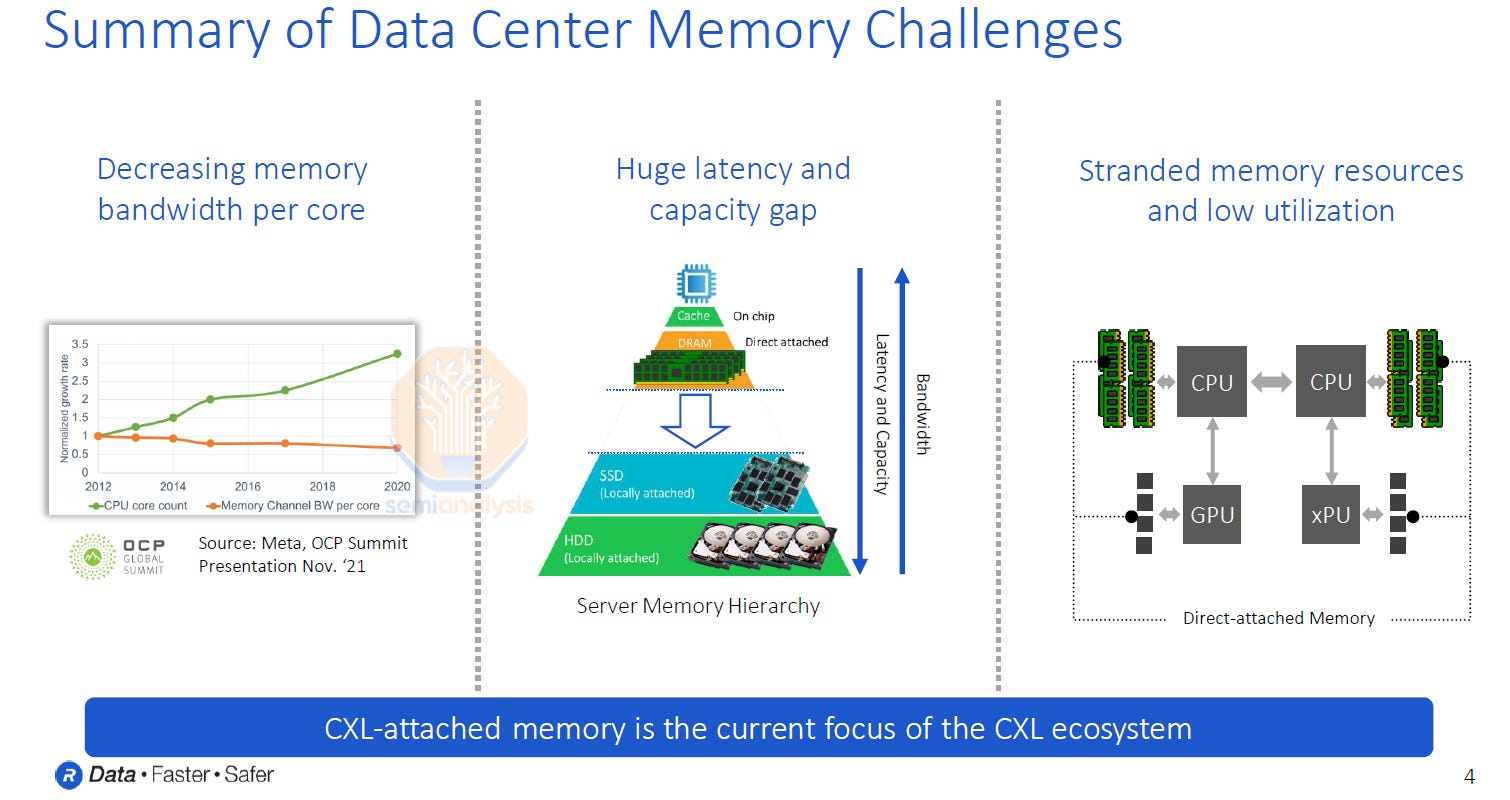
\includegraphics[width=0.9\textwidth]{cxl_vs_competition_timeline.png}
\caption{CXL 与竞争标准的演进时间线对比（来源：SemiAnalysis）}
\label{fig:cxl_timeline}
\end{figure}

\subsection{异构计算的驱动力}

SemiAnalysis 提出了一个深刻的分析框架：摩尔定律放缓与芯片设计成本飙升，共同推动了\textbf{异构计算}的必然性。

\begin{keypoint}[异构计算的逻辑]
\begin{itemize}
    \item 摩尔定律下，每个增量晶体管用于通用 CPU 性能的回报\textbf{递减}
    \item 专用 ASIC 能用更少的晶体管在特定任务上提供 \textbf{10 倍以上}的性能提升
    \item 但是为每种工作负载设计专用芯片\textbf{成本过高}——光罩成本、验证成本持续飙升
    \item \textbf{最优解}：为「计算类别」（classes of computation）设计芯片，通过标准化互连按需组合
\end{itemize}
\end{keypoint}

\begin{transbox}
\textbf{Gordon Moore 在 1965 年原始论文中的远见：}

「将小型功能单元分别封装和互连，构建大型系统可能在经济上更为合理。大型功能单元的可用性，结合功能化设计和构建，应该使大型系统制造商能够快速且经济地设计和构建各种设备。」

—— Gordon Moore, \textit{“Cramming more components onto integrated circuits”}, 1965
\end{transbox}

\begin{analysisbox}
\textbf{数据中心成为新的计算单元}：这种变化将计算单元从单个芯片或服务器提升到\textbf{整个数据中心}。对 CXL 在数据中心影响的准确理解和判断，将成为半导体投资领域最重要的超额收益（Alpha）来源。
\end{analysisbox}

\subsection{数据中心的内存危机}

SemiAnalysis 指出了数据中心面临的根本性内存问题：

\begin{keypoint}[内存三大矛盾]
\begin{enumerate}[label=(\arabic*)]
    \item \textbf{核心数激增，内存带宽/核心下降}：自 2012 年以来，核心数快速增长，但内存带宽每核心却在下降
    \item \textbf{DRAM 与 SSD 之间存在巨大的延迟和成本鸿沟}：缺乏中间层
    \item \textbf{内存利用率极低}：Microsoft 声明服务器成本的 50\% 来自 DRAM，但高达 \textbf{25\% 的 DRAM 是闲置的（stranded）}——这相当于 Microsoft Azure 总服务器成本的 \textbf{12.5\%} 在白白浪费
\end{enumerate}
\end{keypoint}

\begin{figure}[htbp]
\centering
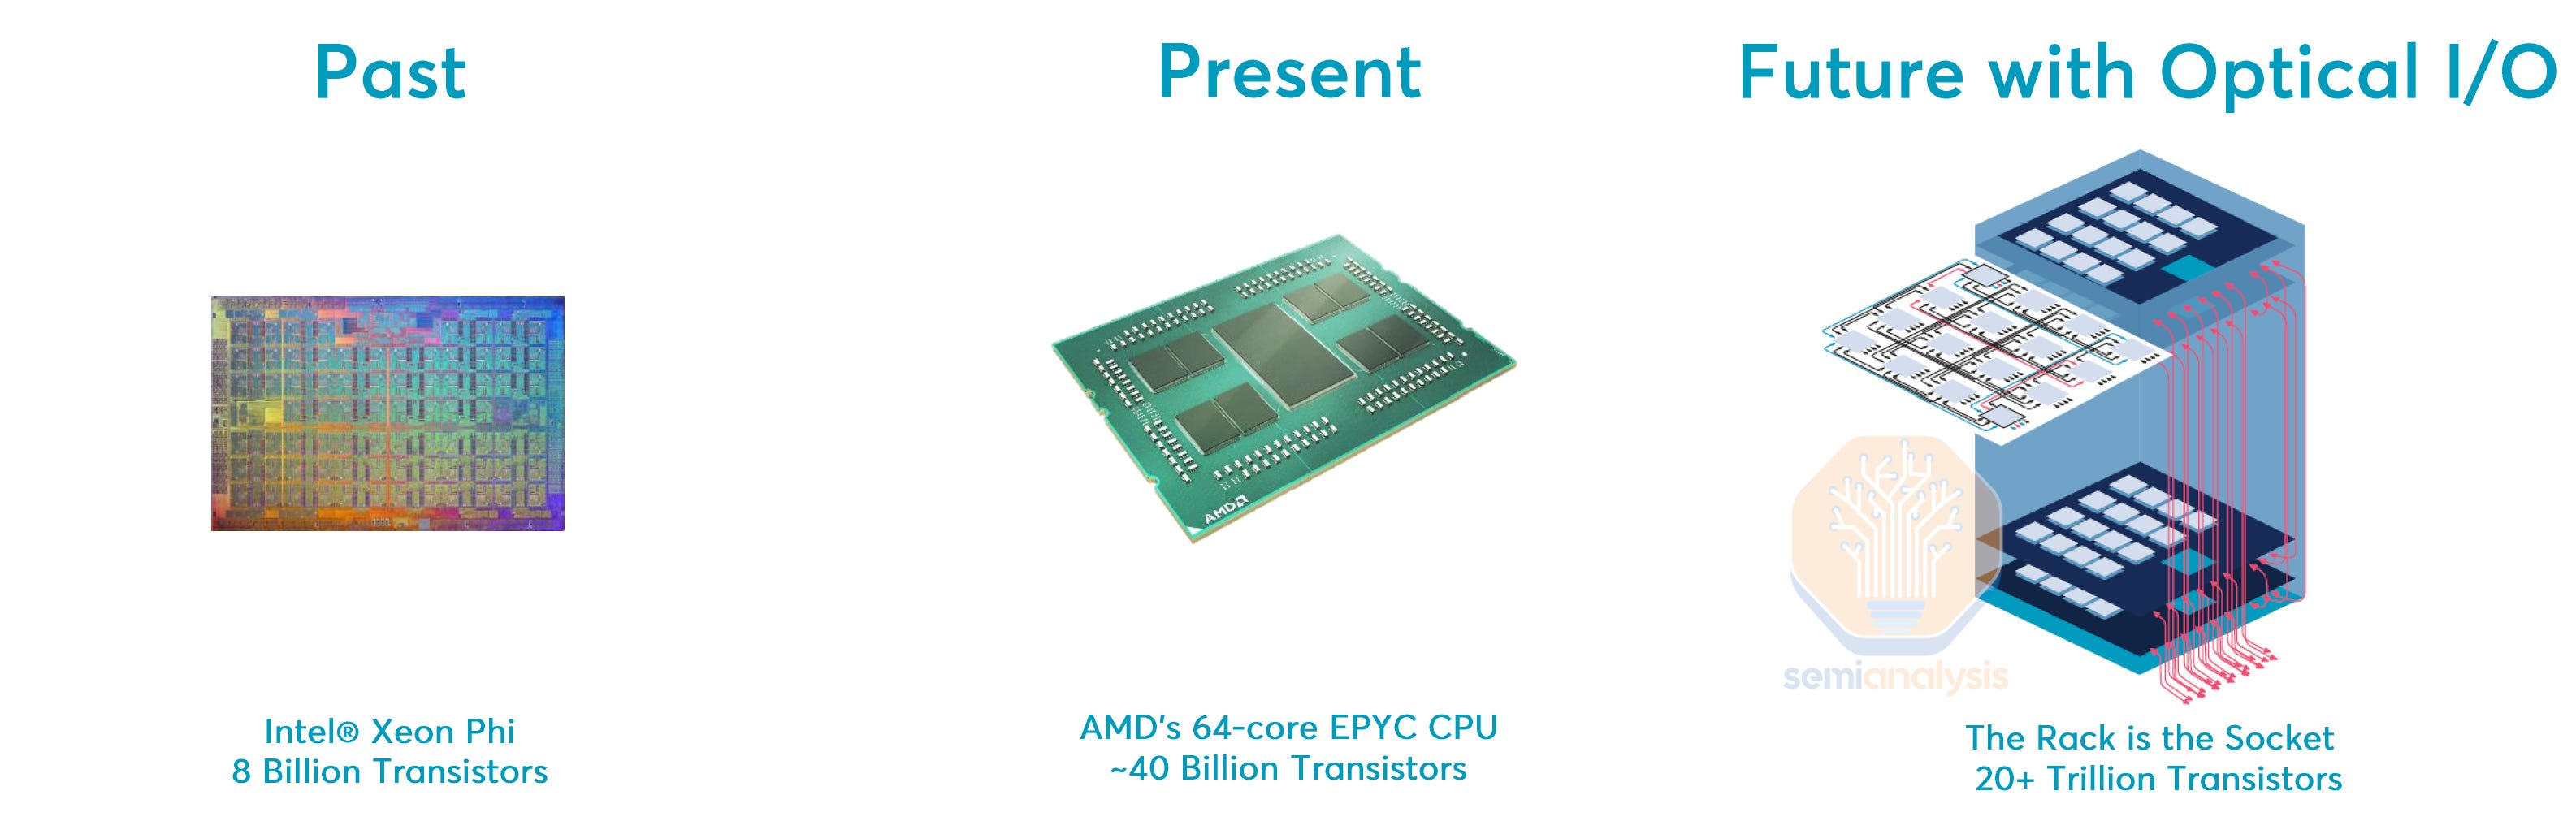
\includegraphics[width=\textwidth]{cxl_memory_bandwidth_core_trend.png}
\caption{内存带宽每核心持续下降趋势（来源：SemiAnalysis）}
\label{fig:mem_bw_core}
\end{figure}

\subsection{可组合服务器架构：数据中心圣杯}

\begin{keypoint}[可组合架构的核心思想]
将服务器拆分为各种组件（CPU、内存、加速器、网络），放置在资源池中，这些资源可以根据工作负载需求\textbf{动态分配}。数据中心机架成为计算单元——客户可以为特定任务选择任意数量的核心、内存和 AI 处理能力。云服务提供商可以根据客户实际运行的负载类型\textbf{动态分配资源}，并\textbf{仅按使用量收费}。
\end{keypoint}

这是服务器设计和云计算的\textbf{圣杯（Holy Grail）}。实现这一愿景的复杂工程问题中，许多都围绕着\textbf{构建互连网络的延迟和成本}。这必须被严格审视，但\textbf{协议必须先行}——这正是 CXL 2.0 和 3.0 带来的东西。

\subsection{CXL 2.0：交换与内存池化}

\begin{figure}[htbp]
\centering
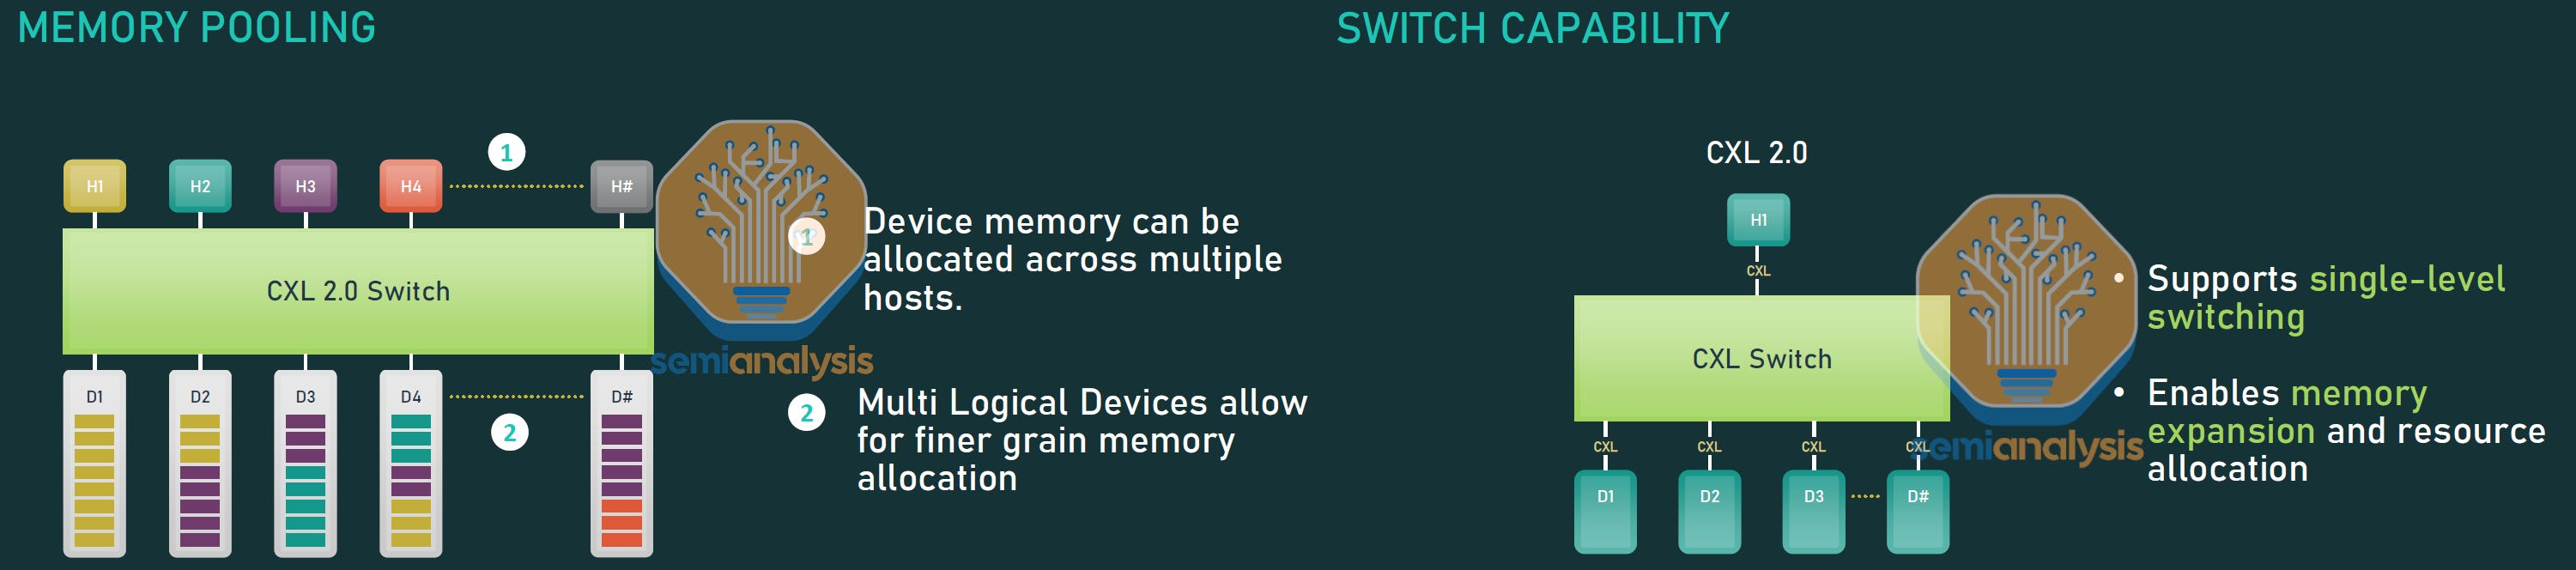
\includegraphics[width=\textwidth]{cxl_memory_pooling_architecture.png}
\caption{CXL 2.0 内存池化架构（来源：SemiAnalysis）}
\label{fig:cxl2_pooling}
\end{figure}

SemiAnalysis 对 CXL 2.0 架构的解读：

\begin{itemize}
    \item 多个主机连接至 CXL 交换机
    \item 交换机连接各种设备：SLD（单逻辑设备）或 MLD（多逻辑设备）
    \item MLD 被设计为耦合到多个主机用于内存池化，在系统中表现为多个 SLD
    \item \textbf{Fabric Manager（FM）} 在控制平面中，是资源编排器，分配内存和设备。它不需要高性能，因为它从不接触数据平面
    \item 如果 CXL 设备是\textbf{多头（multi-headed）}并连接到多个主机的根端口，也可以在没有交换机的情况下实现
\end{itemize}

\begin{keypoint}[Microsoft 验证结果]
Microsoft 的演示表明，通过内存池化可以\textbf{减少 10\% 的 DRAM 部署}，并\textbf{节省 5\% 的总服务器成本}。这还只是第一代 CXL 方案（未使用 CXL 交换机）的效果。
\end{keypoint}

\subsection{CXL 3.0：从服务器到机架的飞跃}

SemiAnalysis 指出 CXL 3.0 的核心变化：

\begin{keypoint}[CXL 3.0 的本质变革]
\textbf{从主从模型（Host-Device）转变为对等网络}：CPU 不再是"主机"，而是网络上的另一个设备节点。核心特性：
\begin{enumerate}[label=(\arabic*)]
    \item \textbf{多级交换拓扑}：从 CXL 2.0 的单一 Fan-out 扩展到 Leaf/Spine、全互联等拓扑
    \item \textbf{设备/主机/交换机/端口理论上限 4096 个}
    \item \textbf{单根端口支持所有设备类型混搭}：此前一个根端口只能访问一种设备类型
    \item \textbf{内存共享（Memory Sharing）}：多个主机和加速器可在同一数据集上\textbf{协作}，无需不必要的数据搬移和重复
    \item \textbf{设备间直接通信（P2P）}：GPU 可直接通信，无需经过主机
\end{enumerate}
\end{keypoint}

\subsubsection{内存共享的实际应用价值}

\begin{analysisbox}
\textbf{例：AI 推荐系统（DLRM）}

Google、Meta 等公司使用的数十亿参数深度学习推荐系统：
\begin{itemize}
    \item \textbf{当前问题：} 相同的模型数据在\textbf{多台服务器中重复存储}
    \item \textbf{CXL 3.0 方案：} 大型 AI 模型可驻留在\textbf{少量中心内存设备}中，多个设备同时访问
    \item \textbf{额外优势：} 模型可用实时用户数据持续训练，更新通过 CXL 交换网络推送
    \item \textbf{收益：} DRAM 成本可降低\textbf{一个数量级}，性能同时提升
\end{itemize}
\end{analysisbox}

\begin{figure}[htbp]
\centering
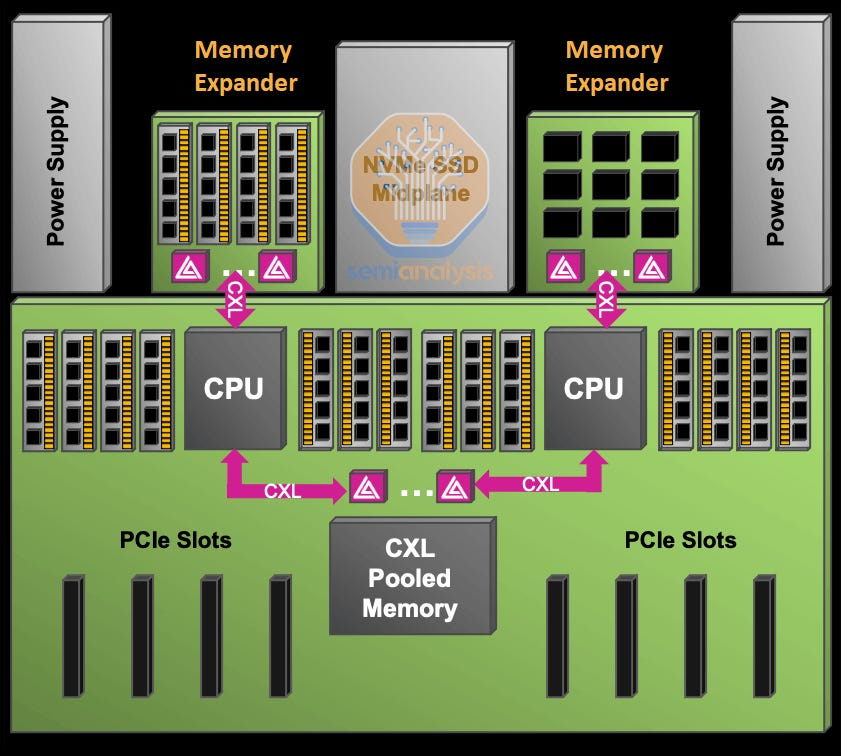
\includegraphics[width=0.85\textwidth]{cxl_memory_sharing_timeline.png}
\caption{内存共享技术演进时间线（来源：SemiAnalysis）}
\label{fig:mem_sharing}
\end{figure}

\begin{figure}[htbp]
\centering
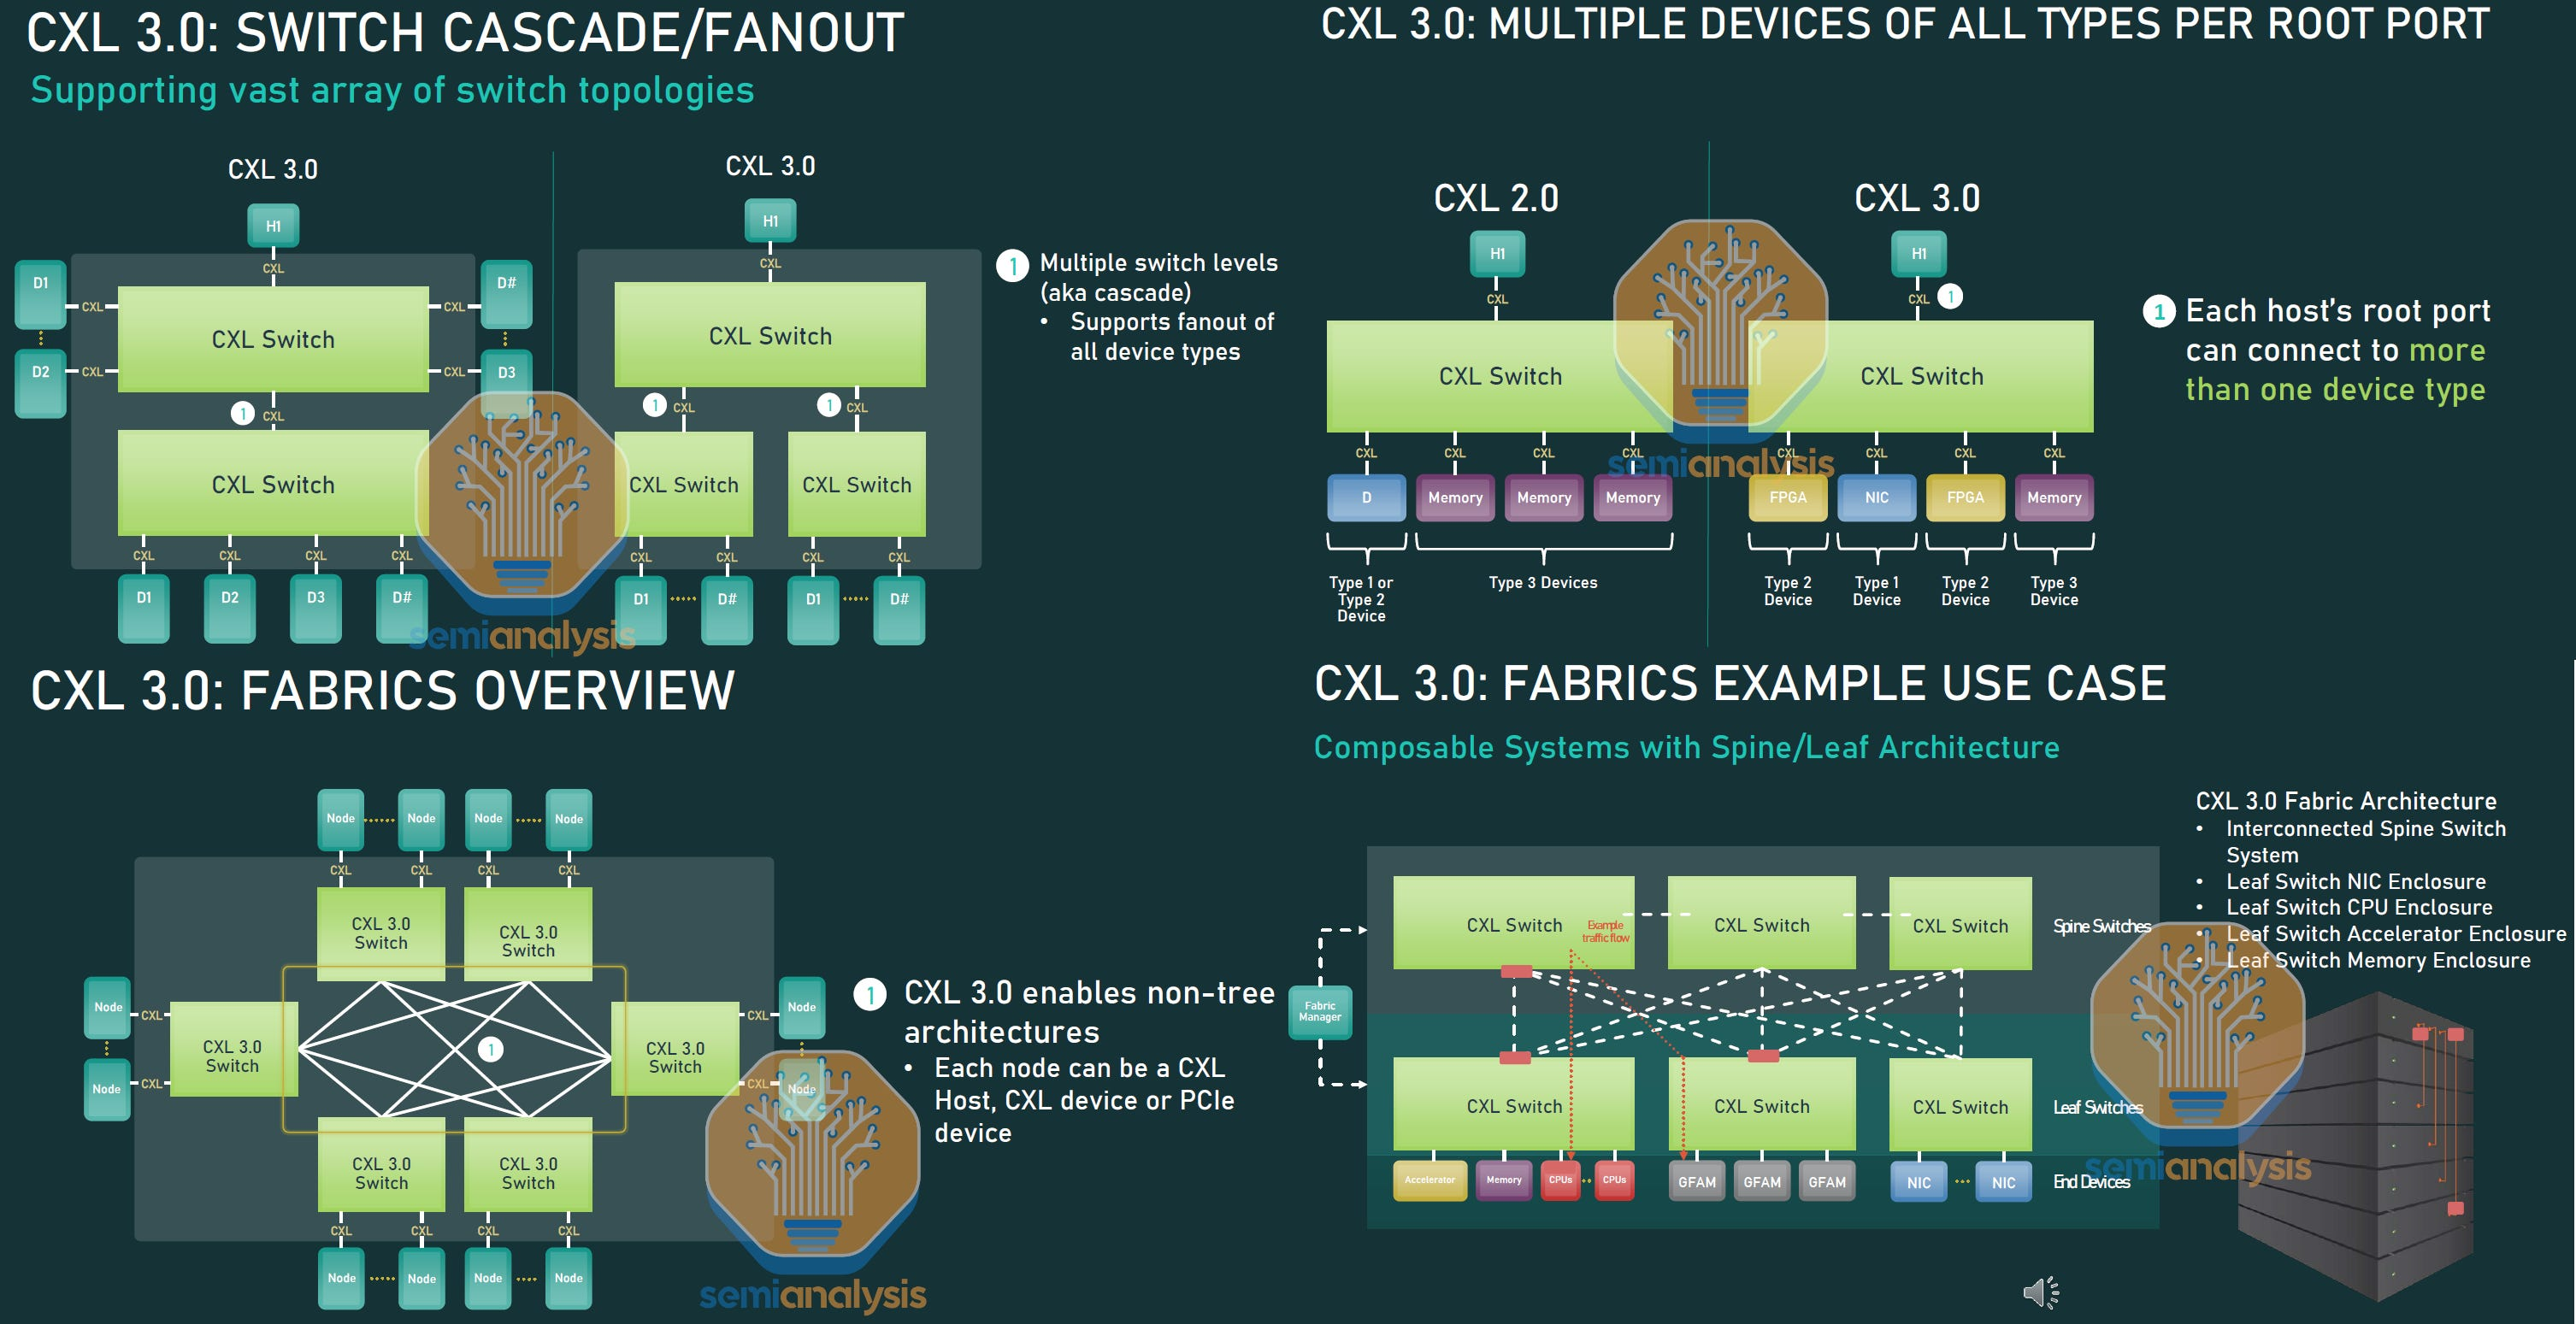
\includegraphics[width=\textwidth]{cxl_dram_savings_chart.png}
\caption{CXL 各代技术带来的 DRAM 节省潜力（来源：SemiAnalysis）}
\label{fig:dram_savings}
\end{figure}

\begin{keypoint}[DRAM 节省的经济价值]
\begin{itemize}
    \item \textbf{第一代内存池化（CXL 2.0）：} 可减少总 DRAM 需求约 \textbf{10\%}
    \item \textbf{低延迟内存池化：} 多租户云场景中可节省约 \textbf{23\%}
    \item \textbf{内存共享（CXL 3.0）：} 可减少 DRAM 需求超过 \textbf{35\%}
\end{itemize}
这些节省代表着每年数据中心 DRAM 支出中\textbf{数十亿美元}的价值。
\end{keypoint}

\subsection{20 家厂商产品布局（付费内容摘要）}

\begin{figure}[htbp]
\centering
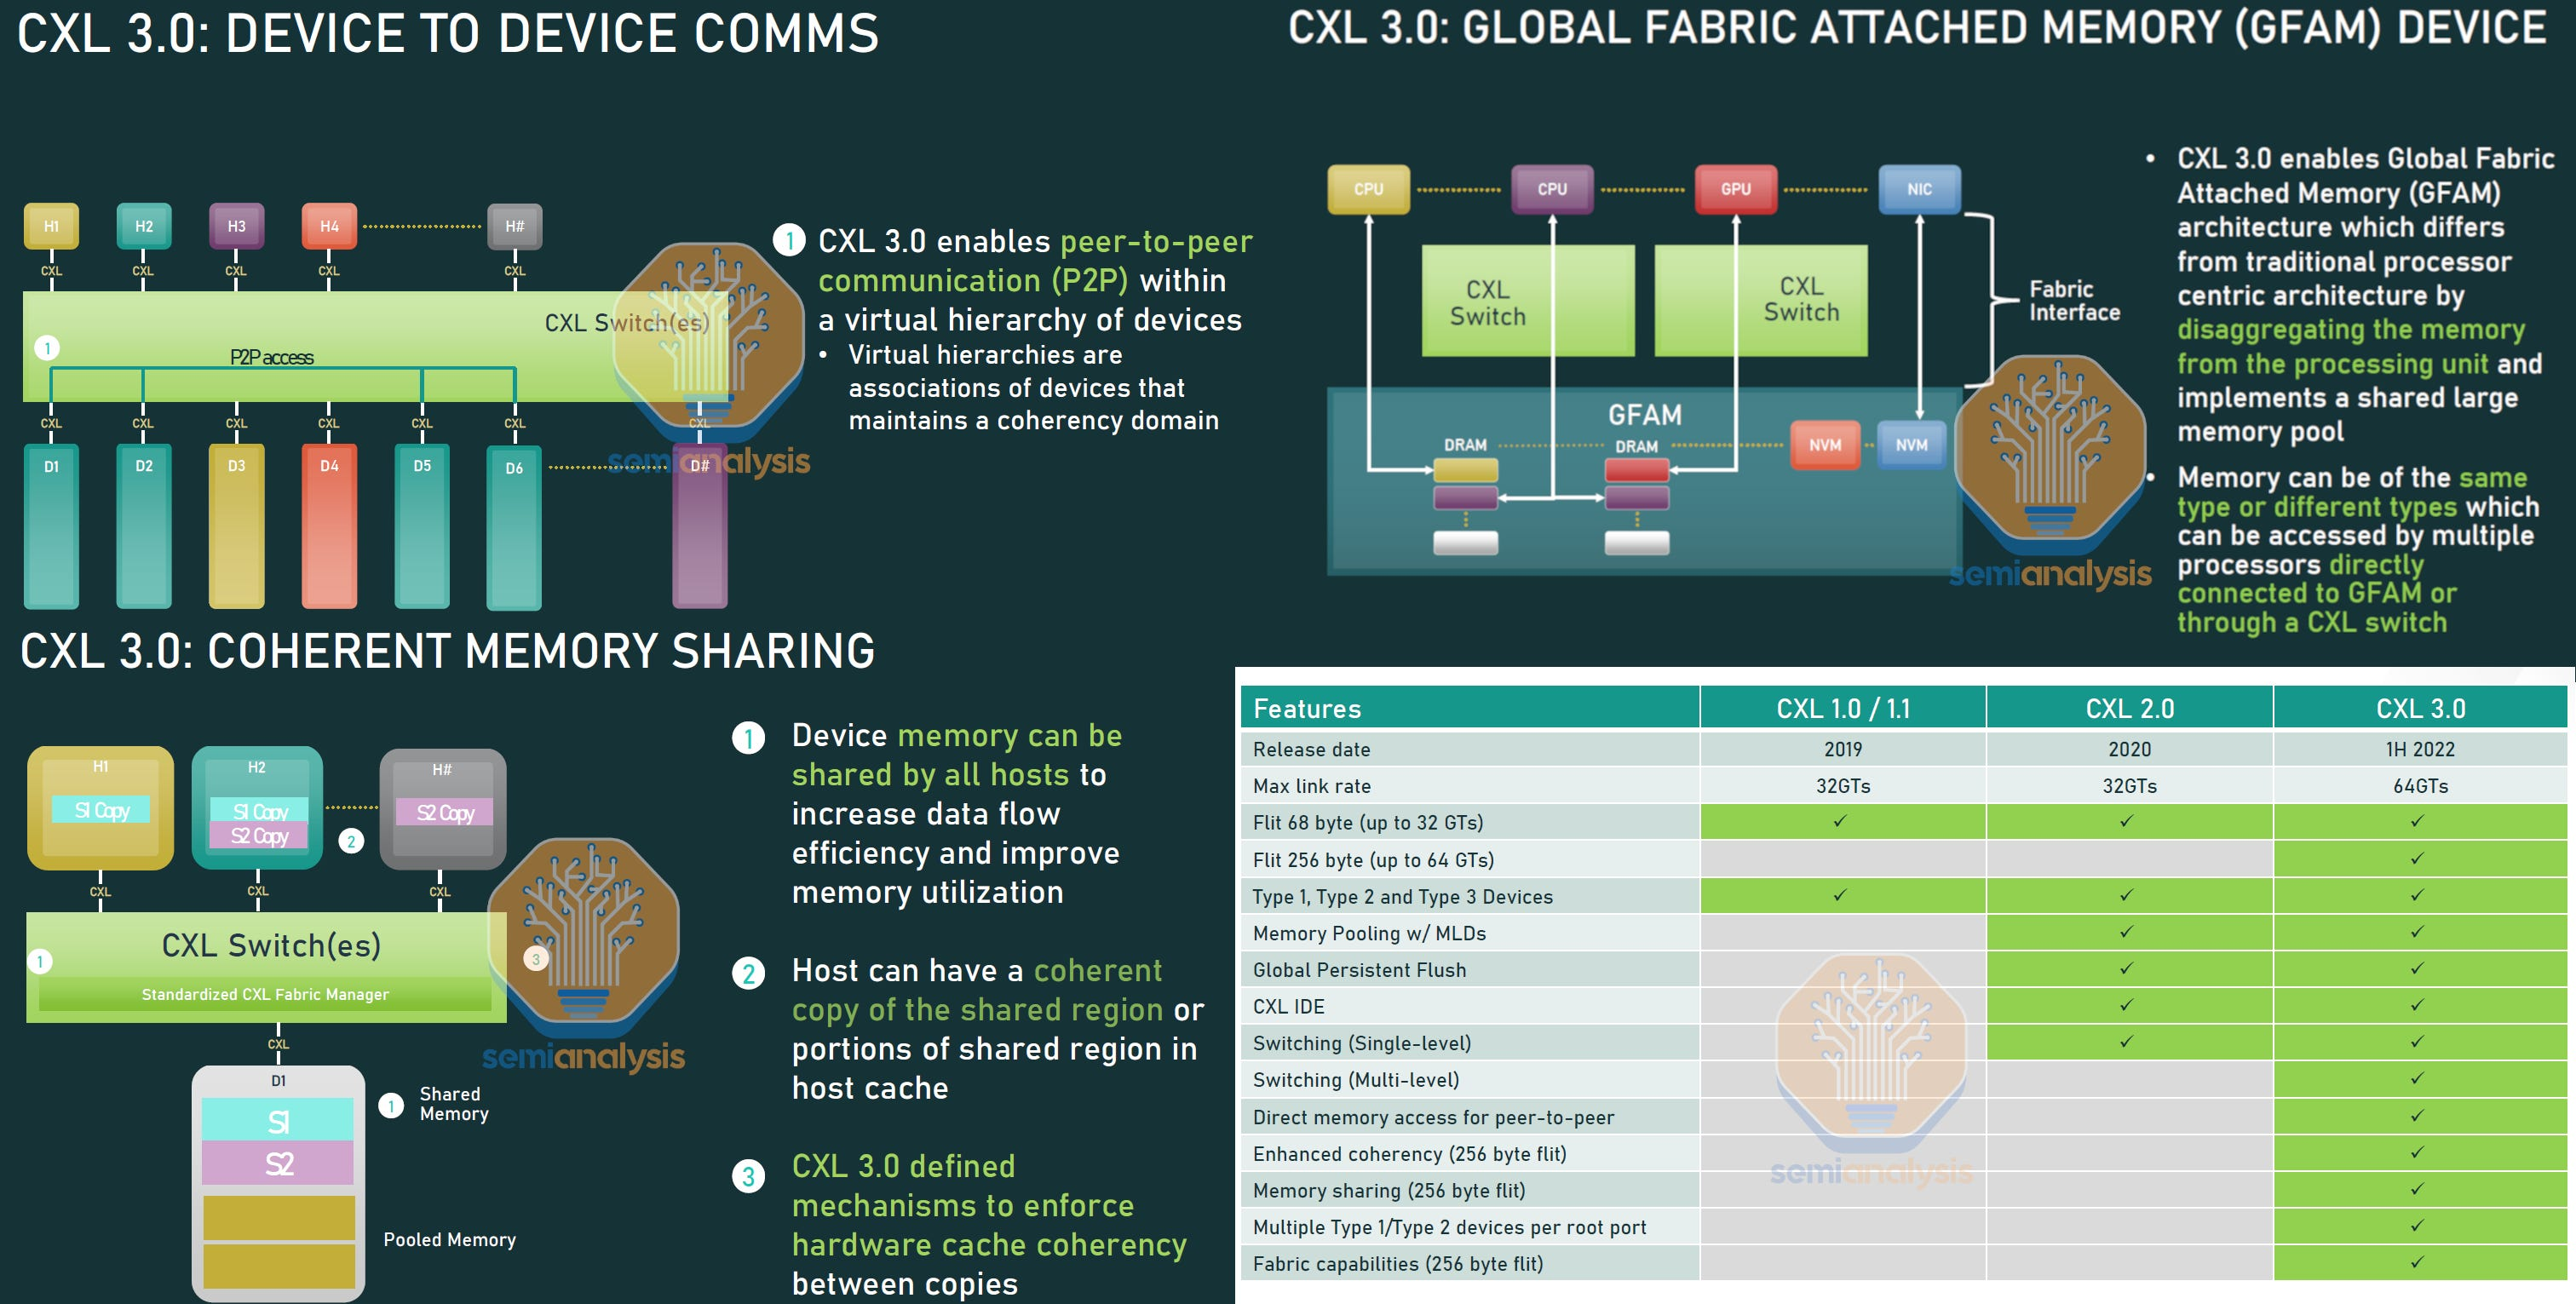
\includegraphics[width=\textwidth]{cxl_product_roadmap.png}
\caption{CXL 产业产品路线图（来源：SemiAnalysis）}
\label{fig:product_roadmap}
\end{figure}

\begin{analysisbox}
SemiAnalysis 在付费部分讨论的 20 家厂商及其 CXL 产品方向：

\begin{tabularx}{\textwidth}{@{}lX@{}}
\toprule
\textbf{类别} & \textbf{厂商与产品方向} \\
\midrule
\textbf{CPU} & Intel（Sapphire Rapids CXL 1.1）、AMD（Genoa CXL 1.1）、Ampere Computing \\
\textbf{GPU/加速器} & NVIDIA、Intel、AMD \\
\textbf{内存} & Samsung、SK Hynix、Micron（CXL 内存模块/扩展器） \\
\textbf{交换机} & Broadcom、Marvell、Microchip、Montage Technology、Xconn \\
\textbf{内存控制器} & Rambus、Astera Labs、Montage Technology \\
\textbf{DPU/IPU} & Intel（IPU）、NVIDIA（DPU） \\
\textbf{光学互连} & Ayar Labs（共封装光学） \\
\textbf{云厂商} & Microsoft、Google、Meta、Alibaba、HPE \\
\bottomrule
\end{tabularx}

\textbf{注意：} 文章指出 CXL 联盟有超过 200 家成员，但上述 20 家被认为拥有最具影响力的产品和 IP。关于片内互连（On-Package）的内容将在后续 UCIe 相关文章中讨论。
\end{analysisbox}

\subsection{SemiAnalysis 核心观点总结}

\begin{keypoint}[该文对 CXL 的关键判断]
\begin{enumerate}[label=(\arabic*)]
    \item CXL 的产业临界质量已经达到——每家主要半导体和数据中心公司都加入了
    \item 异构计算是大势所趋，CXL 是实现异构计算的标准互连基础设施
    \item 内存是数据中心最大的成本项（50\%），也是最大的浪费源（25\% 闲置），CXL 内存池化/共享解决的是真金白银的问题
    \item CXL 3.0 将互连从服务器级别扩展到整机架/多机架级别，这是质的飞跃
    \item 准确理解 CXL 对数据中心的影响将是半导体投资最重要的 Alpha 来源
\end{enumerate}
\end{keypoint}

\subsection{与 Logic Fruit 文章的互补}

\begin{analysisbox}
两篇文章的互补关系：

\begin{itemize}
    \item \textbf{Logic Fruit 文章：} 技术百科全书路线，详细解释三种协议、三种设备类型、各版本特性，适合作为 CXL 入门/参考
    \item \textbf{SemiAnalysis 文章：} 产业分析路线，从经济学角度分析 CXL 的价值逻辑（内存成本、利用率、异构计算趋势），适合理解 CXL 的商业模式和投资价值
\end{itemize}

两者结合，形成了从\textbf{技术原理到商业驱动力}的完整 CXL 知识体系。
\end{analysisbox}

\begin{tcolorbox}[title=参考来源]
\begin{enumerate}[label={[\arabic*]}]
    \item Logic Fruit Technologies: \textit{Compute Express Link (CXL) - An Ultimate Guide}\newline
    \url{https://www.logic-fruit.com/glossary/compute-express-link/}
    \item SemiAnalysis: \textit{CXL Deep Dive – Future of Composable Server Architecture and Heterogeneous Compute}\newline
    \url{https://newsletter.semianalysis.com/p/cxl-deep-dive-future-of-composable}
\end{enumerate}
\end{tcolorbox}

\end{document}
